%%%%%%%%%%%%%%%%%%%%%%%%%%%%%%%%%%%%%%%%%%%%%%%%%%
%%%%%%%%%%%%%%%%%%%%%%%%%%%%%%%%%%%%%%%%%%%%%%%%%%
%%%%%%%%%%%%%%%%%%%%%%%%%%%%%%%%%%%%%%%%%%%%%%%%%%
% PREAMBLE:

\documentclass[11pt,a2paper,landscape]{article}

%%%%%%%%%%%%%%%%%%%%%%%%%%%%%%%%%%%%%%%%%%%%%%%%%%

\usepackage[noheadfoot,margin=10mm]{geometry}
% width=554mm,height=400mm
\usepackage[utf8]{inputenc}
\usepackage[english]{babel}
\usepackage{graphicx,multicol,color} 
%\usepackage{everyshi,eso-pic,calc,ifthen,wallpaper} 
\usepackage{tikz}
\usepackage{amsmath,amsfonts,amssymb,amsthm}
\usetikzlibrary{automata,arrows,positioning,calc}
\usepackage{mathtools}
\usepackage{caption}
\usepackage{anyfontsize}

%%%%%%%%%%%%%%%%%%%%%%%%%%%%%%%%%%%%%%%%%%%%%%%%%%

\pagestyle{empty}
\definecolor{cola}{rgb}{.99,.93,0}
\definecolor{colb}{rgb}{.8,0,.7}
\definecolor{colc}{rgb}{1,.9,.9}
\DeclarePairedDelimiter\abs{\lvert}{\rvert}

%% boxes to put stuff in ......
%%
%%   (1) transparent boxes --- the background shows through
%%			   #1 = width as fraction of what's available
%%                         #2 = contents (text, formula, picture)
%%                               ... tho pictures are always opaque
%% ---- box for headers --- width = fraction of textwidth 

\newcommand\BoX[2]{\begin{minipage}{#1\textwidth}#2\end{minipage}}
%% ---- box centred in a column --- width = fraction of columnwidth
\newcommand\BOX[2]{\begin{center}
   \begin{minipage}{#1\columnwidth}#2\end{minipage}\end{center}\vfill}
%%
%%   (2) opaque boxes with coloured background and outline frame
%%                         #1 = width as fraction of what's available
%%                         #2 = contents (text, formula, picture)
%%                         #3 = background colour
%%                         #4 = frame colour
\setlength\fboxrule{2pt} %% = width of frame lines round boxes
\setlength\fboxsep{5pt}  %% = spacing round box contents
%% ---- box for headers --- width = fraction of textwidth 
\newcommand\cBoX[4]{\fcolorbox{#4}{#3}{%
	\begin{minipage}{#1\textwidth}#2\end{minipage}}}
%% ---- box centred in a column --- width = fraction of columnwidth
\newcommand\cBOX[4]{\begin{center}\fcolorbox{#4}{#3}{%
 \begin{minipage}{#1\columnwidth}#2\end{minipage}}\end{center}\vfill}


%% for e.g. picture and text side-by-side in a column
%%   n.b. this command must be inside a \BOX or a \cBOX
\newcommand\sidebyside[2]{\BoX{.485}{#1}\BoX{.485}{#2}}

\renewcommand\familydefault{\sfdefault}

\newtheorem{definition}{Definition}[section]
\newtheorem{exmp}{Example}[section]
\newtheorem*{theorem*}{Theorem}

\setlength\columnsep{10mm}  %%%% column separation

%%%%%%%%%%%%%%%%%%%%%%%%%%%%%%%%%%%%%%%%%%%%%%%%%%
%%%%%%%%%%%%%%%%%%%%%%%%%%%%%%%%%%%%%%%%%%%%%%%%%%
%%%%%%%%%%%%%%%%%%%%%%%%%%%%%%%%%%%%%%%%%%%%%%%%%%
% DOCUMENT

\begin{document}
\tikz[remember picture,overlay] \node[inner sep=0pt] at (current page.center)
{ 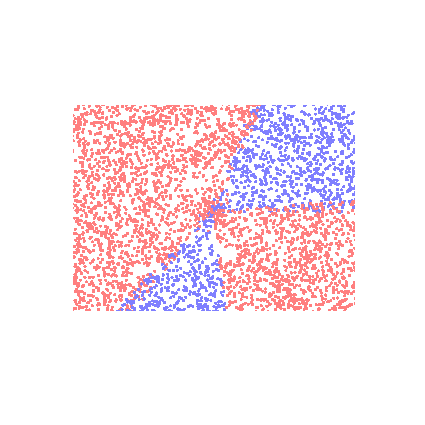
\includegraphics[width=\paperwidth,height=\paperheight]{spiral3.pdf}};

\begin{tikzpicture}[remember picture, overlay]
  \node [anchor=north west, inner sep=1cm]  at (current page.north west)
     {
\includegraphics[height=3cm]{university}};
\end{tikzpicture}
\hfill
\cBoX{0.5}{\color{blue}\centering
\vspace{1ex}
{\fontsize{1.8cm}{2cm}\selectfont{\textsc{Interacting Particle Systems}}}
\vspace{1ex}
}{white}{white}
\hfill
\cBoX{.2}{\color{red}
\centering
\huge
\textit{James Thomas Ayre\\
	 Supervisor: Dr. Ostap Hryniv}
}{white}{white}
\vspace{0.5in} 

%%%%%%%%%%%%%%%%%%%%%%%%%%%%%%%%%%%%%%%%%%%%%%%%%%
%%%%%%%%%%%%%%%%%%%%%%%%%%%%%%%%%%%%%%%%%%%%%%%%%%
%%%  now the body material in 3 columns of stacked boxes
%%      ... use \BOX and/or \cBOX here

\begin{multicols*}{3}
\setlength\fboxrule{1pt} 

%%%   to get more in, try say 4 columns with smaller-sized type
%%%  BUT -- for easy reading 
%%%               use no more than about 66 characters per line
%%%%   .... and choose a size of type that 
%%%%              looks OK expanded from A4 to A2
% \tiny
\small

%%%%%%%%%%%%%%%%%%%%%%%%%%%%%%%%%%%%%%%%%%%%%%%%%%

\fboxsep=5.5pt
\cBOX{0.97}{\section*{Introduction}
Interacting Particle Systems is an area of Probability, that spans several fields of study. 
Typically one starts with a countable number of particles, which would evolve as independent 
Markov chains on some countable state space $I$, and imposes a local interaction between 
these particles. This means that the evolution of an individual particle on $I$ no longer has the 
Markov property. Understanding how these systems develops over time is now much more 
involved.
\vspace{1ex}

While the motivation for Interacting Particle Systems initially came from problems in 
statistical mechanics and from trying to understand phase transition, the area is now 
widely applicable to other areas such as population evolution, modelling infections, 
modelling computer viruses, and behavioural systems.
\vspace{1ex}

We consider continuous time Markov processes, denoted $\eta_{t}$, in a state space 
$S=\{0,1\}^{I}$ where $I$ is the countable collection of sites. The interpretation of the values 
$0,1$ changes for various models, for example they could denote whether a particle occupies 
a particular site. The dynamics of these processes are specified by transition 
rates between states.
\vspace{1ex}



}{white}{white}

%%%%%%%%%%%%%%%%%%%%%%%%%%%%%%%%%%%%%%%%%%%%%%%%%%

\vspace{-0.5cm}
\cBOX{0.97}{\section*{Processes and Models}
There are lots of different types of processes and models, such as the Richardson growth
model, the contact process, the voter model and the exclusion process. The interactions on
these models can lead to some surprising behaviour. In particular we will concentrate on the
behaviours of the Richardson growth model and the voter model when the set of sites 
$I = \mathbb{Z}^{d}$.

\subsection*{Richardson growth model}
We consider a process with $I= \mathbb{Z}^d$, and call $x \in \mathbb{Z}^{d}$ occupied if $\eta_{t}(x)=1$
and vacant if $\eta_{t}(x)=0$. The rate at which there is a change of value at site $x$ is given by a rate function
\begin{equation*}
c(x, \eta)=
\begin{cases}
\mbox{\phantom{ZZ.}}0 & \mbox{ if } \eta(x)=1\\
\sum\limits_{y: |x-y|=1}\eta(y) & \mbox{ if } \eta(x)=0 
\end{cases}
\end{equation*}
where $\eta \in S$. Here a site, once occupied by a particle, remains occupied for all time and a vacant site is
occupied at a rate proportional to the number of occupied neighbours. 
Let $\xi_{t} = \{x \in \mathbb{Z}^{d}: \eta_{t}(x)=1\}$ and if $\xi_{0}=A\subset \mathbb{Z}^{d}$ 
are the initially occupied sites we write $\xi_{t}^{A}$. We can only add points to $\xi_{t}^{A}$, 
so it grows to cover the entire lattice.
\vspace{1ex}

One can think of this as a crude model for the growth of some population.
The situation for $d=1$ is relatively simple, however for $d \geq 2$ there are different paths 
between sites, so \textit{a priori} it is not clear how $\xi_{t}^{A}$ grows.

\subsection*{Voter model}
Taking $I= \mathbb{Z}^{d}$ we consider $x \in \mathbb{Z}^{d}$ to be an individual with an opinion $\eta_{t}(x)=1$
if they are in favour of some issue and $\eta_{t}(x)=0$ if they are not. The rate function is given by
\begin{equation*}
c(x, \eta)=
\begin{cases}
\sum\limits_{y: |x-y|=1}\frac{1}{2d}\eta(y) & \mbox{ if } \eta(x)=0\\
\\
\sum\limits_{y: |x-y|=1}\frac{1}{2d}(1-\eta(y)) & \mbox{ if } \eta(x)=1
\end{cases}
\end{equation*}
The interpretation is that an individual changes their opinion at a rate proportional to the number
of neighbours with a 

different opinion. This is a particular case of a class of models called spin systems, but we will see it also has 
a useful dual process that can be used to give a more comprehensive analysis than for other spin systems.
\vspace{1ex}
 
The voter model can be used to model changing territories of two populations or, as the name suggests, opinions
for or against some topic of interest. One would like to know if there are limiting distributions, and what changes for
different values of $d$.

\subsection*{Contact process}
It will be useful to have a definition for the discrete version of the contact process on $\mathbb{Z}$. 
The process $\zeta_{n}$, is given by a Markov process such that the following properties hold for $x \in \mathbb{Z}$: 
\begin{center}
\begin{itemize}
	\item[(a)]  $\zeta_{n-1}(x)=\zeta_{n-1}(x-1)=0 \Rightarrow \zeta_{n}(x)=0$;
	\item[(b)] $\zeta_{n-1}(x)=1 \mbox{ or } \zeta_{n-1}(x-1)=1 \Rightarrow \zeta_{n}(x)=1$ with probability $p$;
	\item[(c)] At each time step, decisions on sites are made independently.
\end{itemize}
\end{center}


%\subsection*{Contact Process}
%We consider an undirected $G=(V,E)$ whose vertices have bounded degrees. For the contact process on 
%a graph with parameter $\lambda$ on $G$ we take $I=V$. Each vertex represents an individual, which we call 
%infected if $\eta_{t}(x)=$ and healthy if $\eta_{t}(x)=0$. Infected individuals recover independently at rate $1$
%and infect neighbouring healthy vertices at a rate $\lambda$. This gives the following rate function
%\begin{equation*}
%c(x, \eta)=
%\begin{cases}
%1 & \mbox{ if } \eta(x)=1\\
%\lambda \sum_{y: |x-y|=1}\eta(y) & \mbox{ if } \eta(x)=0
%\end{cases}
%\end{equation*}
%The contact process can be used to model things like infections in populations, and the spread of computer
%viruses. If the graph is finite the infection will die off almost surely, but we can ask questions about the 
%survival time of the process under various conditions. We can also ask questions about the long time 
%behaviour of the process on infinite graphs such as lattices.

%\subsection*{Exclusion Process}
%The exclusion process is slightly different from the previous processes. Here two coordinates of $\eta_{t}$
%change at a time. Particles move on $I$ in the following way.
%\begin{itemize}
%	\item[(a)] At most one particle occupies a site $x \in I$;
%	\item[(b)] A particle at $x$ waits for a time $\sim Exp(1)$ and then chooses a site $y \in I$ with probability
%	$p(x,y)$ given by the transition probabilities for a discrete time Markov chain on $I$;
%	\item[(c)] If $y$ is vacant at that time, the particle moves to $y$, otherwise it remains at $x$.
%\end{itemize}
%Once again $\eta(x)=1$ corresponds to occupation and $\eta(x)=0$ corresponds to vacancy.
}{white}{white}

%%%%%%%%%%%%%%%%%%%%%%%%%%%%%%%%%%%%%%%%%%%%%%%%%%

\cBOX{0.97}{\section*{Richardson Growth Model}
This model is constructed by attaching independent Poisson Processes $T_{n}^{(x,y)}$
of rate $1$ for each of its $y$ neighbours, where
$n$ denotes the $n$\textsuperscript{th} arrival, to $x$. If at time $T_{n}^{(x,y)}$ we have $x \in \xi_{t}$ 
and $y \notin \xi_{t}$ we add $y$ to $\xi_{t}$.
\vspace{1ex}

Take $d=1$, $A=\{0\}$ and let $t(n)=\inf\{t : n \in \xi_{t}^{\{0\}}\}$, that is, $t(n)$ is the time taken 
for $n \in \mathbb{Z}$ to become occupied. Suppose $n>0$, then the only way to occupy $n$ 
is to first occupy $1,2,\cdots,n-1$ successively. The interarrival times
are exponentially distributed with parameter 1, and the memoryless property of the exponential
distribution gives us that each successive occupation is independent. Hence by an application 
of the strong law of large numbers we get that $t(n)/n \rightarrow 1$ almost surely. So we can 
see that $\xi_{t}$ grows somewhat linearly when $d=1$.

Now for $d \geq 1$ define a thickened version of our set of occupied sites, $\xi_{t}^{\{0\}}$, as follows
\begin{equation*}
\bar{\xi}_{t}^{\{0\}} := \Big\{ x + y : x \in \xi_{t}^{\{0\}}, y \in \Big[-\frac{1}{2},\frac{1}{2}\Big]^{d} \Big\}
\end{equation*}
This gives rise to the following result for the limiting shape.
}{white}{white}

%%%%%%%%%%%%%%%%%%%%%%%%%%%%%%%%%%%%%%%%%%%%%%%%%%

\columnbreak
\cBOX{0.97}{\subsection*{}
\begin{theorem*}
Let $\epsilon>0$ be given, then $\exists$ a convex set $A$ s.t.
\begin{equation*}
P\Big[(1-\epsilon)tA \subset \bar{\xi}_{t}^{\{0\}} \subset (1+ \epsilon)tA\Big] \rightarrow 1 
\mbox{ as } t \rightarrow \infty
\end{equation*}
\end{theorem*}

If $\xi_{t(x)+u}^{(x,t(x))}$ is the set of sites that can be reached
after time $u$ from $x$ at time $t(x)$, we define 
$$t(x,y) = \inf\{ u : y \in \xi_{t(x)+u}^{(x,t(x))}\}$$ 
We have that $t(x,y)$ is independent of $t(x)$ by properties 
of the Poisson process and $t(x,y)$ has the same distribution has $t(y-x)$ by translational 
symmetry of the lattice. 
\vspace{1ex}

Taking $n \in \mathbb{Z}$ one can use the subadditive ergodic theorem to obtain that
$t(0,nx)/n \rightarrow$ some limit $\mu(x)$ as $n \rightarrow \infty$, so in particular we have that
$\xi_{t}^{\{0\}}$ grows linearly in each direction. By setting $t(x)= \inf\{t: x \in \bar{\xi}_{t}^{\{0\}}\}$
we extend $t(x)$ to all $x \in \mathbb{R}^{d}$. It is possible to show that
\begin{equation*}
\frac{t(nx)}{n} \rightarrow \mu(x) \mbox{ a.s. } \forall x \in \mathbb{R}^{d}
\end{equation*}
It turns out that $\mu$, given by $\inf_{m\geq 1}\frac{E(t(mx))}{m}$, defines a norm on 
$\mathbb{R}^{d}$. The convex set $A$ in the theorem is given by the unit ball in that norm.
In particular for $\mathbb{Z}^{2}$ we see that $\bar\xi_{t}^{\{0\}}/t$ is, in the
sense of the norm $\mu$, roughly circular. However it is very difficult to compute $\mu$ from
this expression, so it does not really tell us much about how our process is growing.
\vspace{1ex}
 
To get a better feel for the norm and the limiting shape of the growth model we will pass to a 
discrete version of the process on $\mathbb{Z}^{2}$.
}{white}{white}

%%%%%%%%%%%%%%%%%%%%%%%%%%%%%%%%%%%%%%%%%%%%%%%%%%

\cBOX{0.97}{
\subsection*{Understanding the limiting shape}
The discrete version of the Richardson growth model follows the same rules, but if a site is vacant at
time $n$, and at least one of its neighbours is occupied, it becomes occupied with probability $p$.
Decisions at different times and different sites are made independently. Just
as for the continuous case, we have an asymptotic shape result.
\vspace{1ex}

For any $p \in (0,1)$ there exists a norm $\mu_{p}(x)$ on $\mathbb{R}^{2}$, and for any $\epsilon > 0$,
$$P\Big[\{\mu_{p} \leq 1-\epsilon \} \subset \frac{\bar{\xi}_{n}^{\{0\}}}{n} \subset
\{\mu_{p} \leq 1+\epsilon \}\Big] \rightarrow 1 \mbox{ as } n \rightarrow \infty$$

\subsection*{Flat edges}
We identify an embedded discrete contact process given by $\zeta_{n}(x)= \eta_{n}(x,n-x)$, where
$x \in \mathbb{Z}$. It is known for the contact process that $\exists \mbox{\phantom{Z}} p_{0}<1$ such that 
$p>p_{0} \Rightarrow P(\zeta_{n} \not\equiv 0 \mbox{ for all } n) >0$, so the inclusion 
$\{x \in \mathbb{Z}^{2}: \eta_{n}(x) =1\} \supset \{(y,n-y): \zeta_{n}(y)=1\}$ gives us that
for  $P(\zeta_{n} \not\equiv 0 \mbox{ for all } n) >0$
\begin{equation*}
B_{p}:=\{x:\mu_{p}(x) \leq{1}\} \cap \{x: x_{1}+x_{2}=1\} \neq \phi
\end{equation*}
Symmetry arguments yield that $(1/2,1/2) \in B_{p}$, and if we define
$p_{cr} =  \inf\{p: P(\zeta_{n} \not\equiv 0 \mbox{ for all } n) >0\}$, then the result reads that 
for $p>p_{cr}, (1/2, 1/2) \in B_{p} \mbox{ and } \mu_{p}(1/2, 1/2)=1$.
\vspace{1ex}

It can be shown that for $p>p_{cr}$, we have $\partial B_{p} \cap \{x: x_{1}+x_{2}=1\}$
is an interval of length at least $2\sqrt{2}\mbox{\phantom{.}}[p-p_{cr}]$. This means that in the limit of our rescaled
set of occupied points, the boundary has edges that look flat.
\vspace{1ex}

In fact simulations of the discrete Richardson growth model, you see that for $p$ close 
to $1$, the limiting shape is close to a diamond, but as $p$ varies from $1$ to $0$, 
the limiting shape becomes more and more circular.
}{white}{white}

%%%%%%%%%%%%%%%%%%%%%%%%%%%%%%%%%%%%%%%%%%%%%%%%%%

\cBOX{0.97}{\subsection*{Discrete simulations in Python}
Colouring only the boundary, we can see the shape of the rescaled set of occupied points.
\sidebyside{
\hspace{7ex}
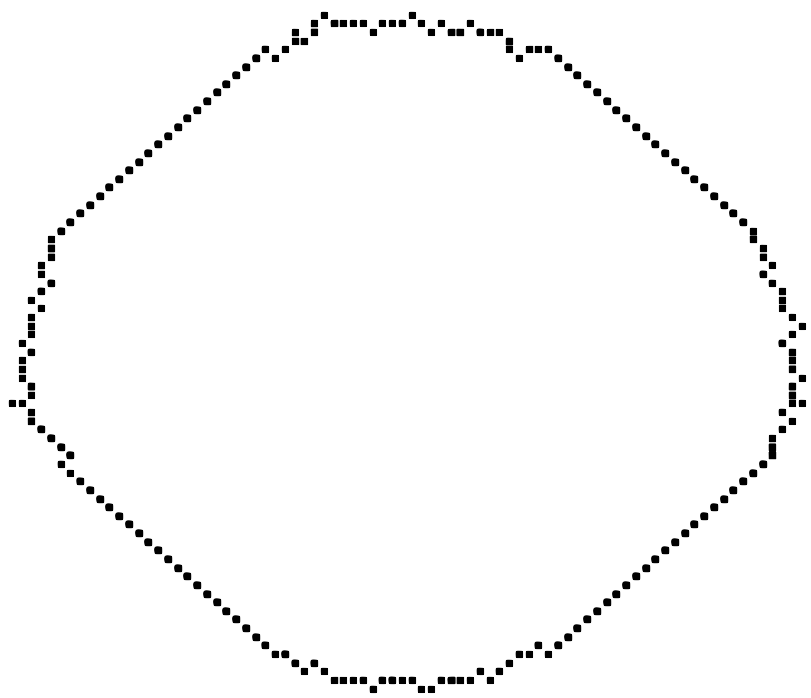
\includegraphics[scale=0.28]{pic2.png}
\captionof{figure}{$n=50$, $p=0.6$}
}
{
\hspace{6ex}
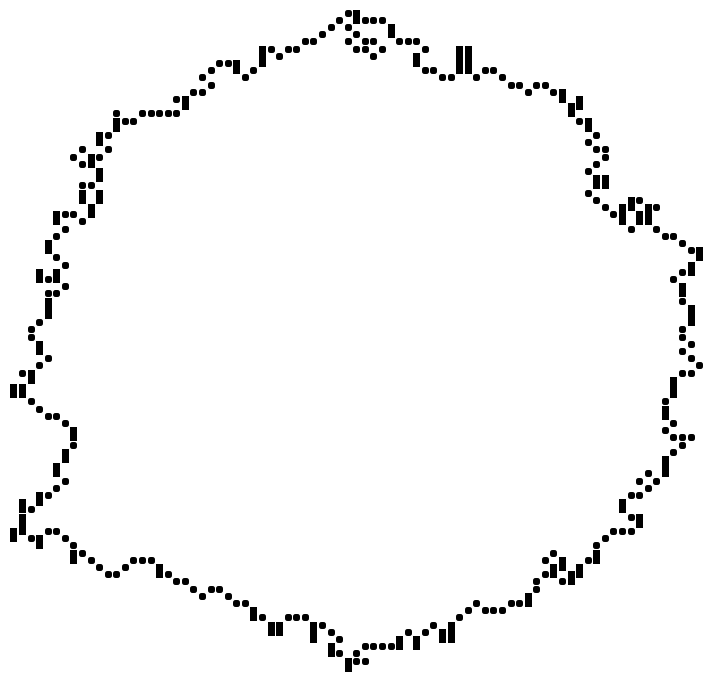
\includegraphics[scale=0.30]{pic1.png}
\captionof{figure}{$n=200$, $p=0.1$}
}
}{white}{white}

%%%%%%%%%%%%%%%%%%%%%%%%%%%%%%%%%%%%%%%%%%%%%%%%%%

\cBOX{0.97}{
\subsection*{The two-type Richardson growth model}
For two different types of particles, type I and type II, on $\mathbb{Z}^{d}$ we define the two-type
Richardson growth model in a similar manner. Vacant sites are occupied by a particle of type I or 
type II at a rate given by the number of neighbours of a given type multiplied by parameters
$\lambda_{1}, \lambda_{2}$ respectively. Once a particle occupies a site, it occupies it for all
future times. Starting from a single occupied site for each type, it is not clear whether the sets of 
occupied sites for each types can both grow to be infinite. For example it can happen that one 
set completely surrounds the other and prevents further growth.
\vspace{1ex}

It is conjectured that for $d \geq 2$, starting from single sites, the probability that the sets of occupied
sites can both grow to infinite size is positive if and only if $\lambda_{1}=\lambda_{2}$. 
\vspace{1ex}

It is known that for all but at most countably many values of $\lambda := \lambda_{2}/\lambda_{1}$,
the probability that both sets of occupied sites can grow to be infinite is $0$.

%\subsection*{Central limit theorem}
%So far we have seen that we have a law of large numbers for $t(nx)$, but we have said nothing about the
%its fluctuations. It can be shown that they are bounded by $\sqrt{n}$, but several simulations have indicated 
%that its fluctuations are more likely to be of order $n^{1/3}$.
}{white}{white}

%%%%%%%%%%%%%%%%%%%%%%%%%%%%%%%%%%%%%%%%%%%%%%%%%%

\columnbreak
\cBOX{0.97}{\section*{Voter Model}
To each $ x \in \mathbb{Z}^{d}$ we attach independent Poisson processes $T_{n}^{x}$ of rate $1$, and 
let $Y_{n}^{x}$ be independent i.i.d. sequences, with $P(Y_{n}^{x}=y)=1/2d$ for all $y$ with $\abs{y}=1$.
The individual $x$ changes their opinion for the nth time at time $T_{n}^{x}$ to that of $x+Y_{n}^{x}$.
The process can be represented graphically on $\mathbb{Z}^{d}\times[0,\infty)$ by drawing arrows
from $(x+Y_{n}^{x},T_{n}^{x})$ to $(x,T_{n}^{x})$, and we also write a $\delta$ at $(x,T_{n}^{x})$
for each $x$ and $n$. 
\vspace{1ex}

There is a path between $(x,0)$ and $(y,t)$ if there is a sequence of times 
$s_{0}=0<s_{1}<s_{2} \cdots <s_{n}< s_{n+1}=t$ and locations $x_{0}=x,x_{1}, \cdots, x_{n}=y$ 
such that there is an arrow between $x_{i-1}$ and $x_{i}$ at time $s_{i}$ and there is no $\delta$ in 
$\{x_{i}\}\times(s_{i},s_{i+1})$. When such a path exists individual $y$ at time $t$ will share the opinion 
of $x$ at time $0$. 
\vspace{1ex}

This can be thought of as fluid flowing up the graph from $\xi_{0}\times \{0\}$, where
$\xi_{t}$ is as in the Richardson growth model. 
Upward motion is stopped whenever the fluid meets a $\delta$ and the fluid also moves in the direction 
of the arrows where possible. That is $$\xi_{t}^{A} = \{y: \exists \mbox{ a path between } (x,0) \mbox{ and } 
(y,t) \mbox{ for some x} \in A\}$$

\sidebyside{
\begin{center}
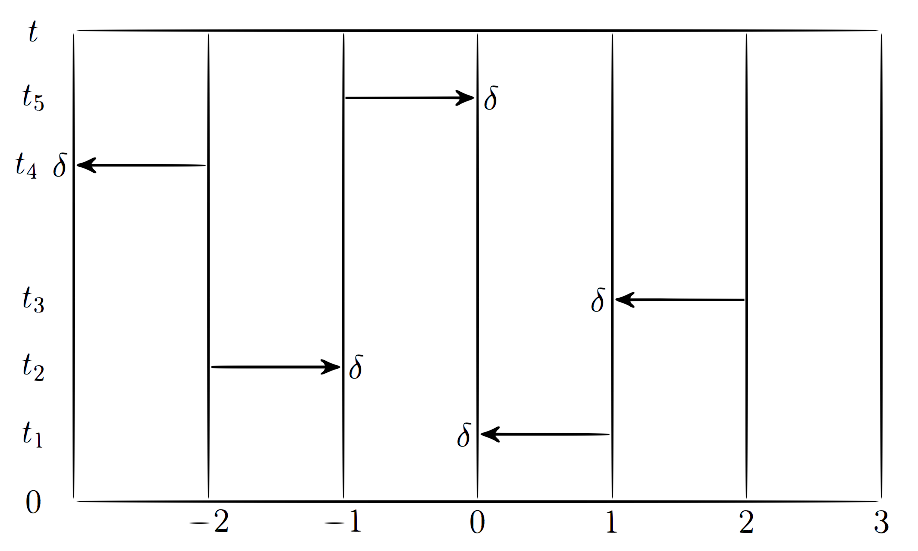
\includegraphics[scale=0.2]{vcon.png}
\end{center}}
{\vspace{1ex}Supposing this graph represents the process for $d=1$, then
the opinion of individual $0$ at time $t$ is the same as that of individual $-2$ 
at time $0$, and if we set $A=\{-2\}$ we get that $\xi_{t}^{\{-2\}}=\{-3,-2,-1,0\}$.

We can define a dual process $\tilde{\xi}_{t}^{B}$ by reversing the direction of 
the arrows, that is
\vspace{-2ex}
$$\tilde{\xi}_{t}^{B} = \{ x:\exists \mbox{ a path between }(y,0)\mbox{ and }(x,t)\mbox{ for some y} \in B\}$$

\vspace{-2ex}
This is distributed in such a way that $P(\xi_{t}^{A}\cap B \neq \phi) = 
P(\tilde{\xi}_{t}^{B} \cap A \neq \phi)$
}

\subsection*{Limiting distributions}
It is easy to see that $\eta \equiv 0$ and $ \eta \equiv 1$ are invariant for the process, as if all
individuals are of the same opinion, nobody can change. However it is not clear that the 
process has other invariant extremal measures.
The trick here is to relate our dual process to a simple random walk, 
which is recurrent in dimension $d=1,2$ and transient for $d \geq 3$. 
\vspace{1ex}

From this we can obtain that the voter model on $\mathbb{Z}^{d}$
reaches a consensus for $d \leq 2$, but for $d \geq 3$ we get a family of limiting distributions. In particular
we get a different limiting distribution for every $p \in [0,1]$ if we start from an initial configuration 
which puts $\eta_{0}(x)=1$ with probability $p$, i.e. the product measure with density $p$.
}{white}{white}

%%%%%%%%%%%%%%%%%%%%%%%%%%%%%%%%%%%%%%%%%%%%%%%%%%

%\cBOX{0.97}{\section*{Contact Process}
%This process can also be constructed graphically. To $x \in I$ attach independent Poisson processes
%$\{T_{n}^{(x,y)}, n \geq 1\}$ of rate $\lambda$ for each neighbour $y$ and $\{U_{n}^{x}, n \geq 1\}$ of
%rate $1$. For the times $T_{n}^{(x,y)}$ draw an arrow from $x$ to $y$ and write at $\delta$ at times
%$U_{n}^{x}$. Paths and $\xi_{t}^{A}$ are defined as they were in the Voter model.

%If we take $I=\mathbb{Z}^{d}$ it is not clear if the process survives. If we take $\lambda \leq 1/2d$
%the maximal rate of infection for any individual is less than its healing rate, and the process will
%die out almost surely.

%In the situation of the finite graph approximate results are known for the expected lifetime of 
%the infection. 
%}{white}{black}

%%%%%%%%%%%%%%%%%%%%%%%%%%%%%%%%%%%%%%%%%%%%%%%%%%

\vspace{-2cm}
\cBOX{0.97}{
\subsection*{Threshold voter model}
The voter model we defined above is in fact a particular case of the linear voter model.
There are nonlinear models such as the threshold voter model. If we intersect $\mathbb{Z}^{d}$
with a compact, convex and symmetric set $X \subset \mathbb{R}^{d}$ we obtain a neighbourhood
$\mathcal{N}=X \cap \mathbb{Z}^{d}$ of $0$. For a positive integer $T$, the threshold model
corresponding to $\mathcal{N}$ and $T$ has rate function
\begin{equation*}
c(x, \eta)=
\begin{cases}
1 & \mbox{ if } \#\{y \in x + \mathcal{N}: \eta(y) \neq \eta(x)\}\geq T\\
0 & \mbox{ otherwise.}
\end{cases}
\end{equation*}
This essentially gives that individuals have an area of effect on the opinions of neighbouring individuals.
While this seems like a minor extension its behaviour can be strange, even in $d=1$. 
For example it is possible for the system to get trapped in a non-trivial extremal measure in the sense that, 
starting from any initial configuration, each $x \in \mathbb{Z}$ will only change its opinion finitely many times.
In the case we say that the process fixates.
If we consider $\mathcal{N}=\{-1,0,1\}$ and $T=2$, the system can become trapped in
$$ \cdots \phantom{Z} 1 \phantom{Z} 1 \phantom{Z} 0 \phantom{Z} 0 \phantom{Z} 1 \phantom{Z} 1
\phantom{Z} 0\phantom{Z} 0\phantom{Z} 1\phantom{Z} 1\phantom{Z} 0\phantom{Z} 0  \phantom{Z} \cdots $$
More generally if $\eta_{t}(x) = \eta_{t}(x+1)$ then these two individuals have the same opinion for all 
future times. In contrast this situation does not arise in linear voter models. In particular

$$ \mbox{ the process fixates when }T > \frac{\#\mathcal{N}-1}{2}$$

In one dimension, if any interval of length $T$ is constant at any time, then individuals
in the interval will never change their opinion, so it is easy to see why it fixates in this case.
In fact for dimension one, when $\mathcal{N}=\{-T,\cdots,T\}$, the limiting distributions are given 
by consensus.
}{white}{white}

%%%%%%%%%%%%%%%%%%%%%%%%%%%%%%%%%%%%%%%%%%%%%%%%%%

\vspace{-2cm}
\cBOX{0.97}{\section*{Final Remarks}
Each of the models presented here can be studied in greater generality, for
various index sets $I$. There are many results for processes taking $I=V$ for 
some vertex set $V$ of a connected undirected graph $G=(V,E)$, whose
vertices have bounded degrees.
\vspace{1ex}

The behaviours of many models, even simple ones such as the Richardson
growth model, can have some very non-trivial properties. While there are 
lots of known results for these models, small changes in the local dynamics 
can lead to completely different global behaviours, which are often difficult
to understand.
}{white}{white}

%%%%%%%%%%%%%%%%%%%%%%%%%%%%%%%%%%%%%%%%%%%%%%%%%%

\vspace{-1.9cm}
\cBOX{0.97}{
\nocite{*}
\bibliographystyle{plain}
\bibliography{poster} 
}{white}{white}
\end{multicols*}
\end{document}

%%%%%%%%%%%%%%%%%%%%%%%%%%%%%%%%%%%%%%%%%%%%%%%%%%
%%%%%%%%%%%%%%%%%%%%%%%%%%%%%%%%%%%%%%%%%%%%%%%%%%
